\begin{comment}
\end{comment}

\chapter{Simulation de circuits quantiques avec les réseaux de tenseurs}
\label{ann:simulation-circuits-quantiques-avec-reseaux-de-tenseurs}

La simulation classique d'états quantiques est tout sauf évidente. Ces états, appartenant à l'espace de Hilbert, sont décrit par des vecteurs d'état de taille exponentielle empêchant ainsi leur caractérisation même pour des systèmes de taille modeste. Cette difficulté, présente dans de nombreux domaines telle l'apprentissage-machine, est aussi connue sous le nom de la \textit{malédiction de la dimensionnalité}. Cependant, la représentation de certains états physiques intéressants contient parfois de l'information superflue ou une structure inhérente. Par exemple, un état quantique général de $n$ qubits requiert en théorie un vecteur d'état à $2^{n}$ bits, mais un état quantique non intriqué nécessite seulement $2n$ bits en raison de l'absence de corrélation. Cette idée a alors mené au développement des méthodes de réseaux de tenseurs pour l'étude de système quantique à plusieurs corps en matière condensé afin d'obtenir une représentation des états quantiques plus efficace. 

Cette annexe décrit seulement en surface les méthodes de réseaux de tenseur. Pour comprendre les différentes méthodes plus en profondeur, de nombreux excellents tutoriels ont été écrits~\cite{bridgemanHandwavingInterpretiveDance2017,biamonteTensorNetworksNutshell2017,bakerMethodesCalculAvec2021}. La section~\ref{sec:reseaux-de-tenseurs} introduit les réseaux de tenseurs ainsi que les principales opérations possibles. Une représentation alternative de ceux-ci, les états en produit de matrices, sont décrit à la section~\ref{sec:mps-mpo} alors que la correspondance entre la simulation de circuits quantiques et la contraction de réseaux de tenseurs est expliqué à la section~\ref{sec:simulation-de-circuits-quantiques}.

%-----------------------------------------------------------------------------%

\section{Réseaux de tenseurs}
\label{sec:reseaux-de-tenseurs}

Un \textit{tenseur} est un tableau multilinéaire de rang, c'est-à-dire un nombre de dimensions, arbitraire encodant une certaine quantité d'information. Par exemple, un scalaire, un vecteur et une matrice correspondent respectivement à un tenseur de rang 0, 1 et 2. Les tenseurs généralisent en outre ces derniers objets en admettant des tenseurs de rang $m$. 

\begin{maindefinition}{Tenseur}{tenseur}
    Un tenseur $T[x_{1}, x_{2}, \dots, x_{m}]$ de rang $m$ avec dimensions $d_{1} \times d_{2} \times \dots \times d_{m}$ est un élément de l'ensemble $\mathbb{C}^{d_{1} \times d_{2} \times \dots \times d_{m}}$.
\end{maindefinition}

Plus formellement,  Pour simplifier la notation, un tenseur s'écrit succinctement comme $T[\varepsilon]$ où $\varepsilon \subseteq \set{ x_{1}, x_{2}, \dots, x_{m} }$. Les tenseurs s'interprètent aussi comme des fonctions définies sur un domaine discret. L'attrait principal des tenseurs est leur représentation géométrique simple, qui permet de visualiser aisément leurs caractéristiques principales et de faciliter leur manipulation. Tout tenseur $T$ se représente par une forme géométrique, où chaque indice $x_{i}$ est représenté par une patte sortant de la forme tel qu'illustré à la figure~\ref{fig:tensor}. Un réseau de tenseurs est une collection de tenseurs $\set{ T_{1}[\varepsilon_{1}], T_{2}[\varepsilon_{2}], \dots, T_{n}[\varepsilon_{n}] }$ partageant certains indices $x_{i}$. La notation en réseaux de tenseurs s'apparente beaucoup à la notation d'Einstein; les sommations sont donc souvent implicites. 

\begin{figure}[h!]
    \centering
    \begin{subfigure}[h]{0.24\textwidth}
        \centering
        \caption{}
        
\includegraphics[width=1\textwidth]{figures/tensor-1.pdf}
        \label{fig:vqcount-circuit-a}
    \end{subfigure}
    \begin{subfigure}[h]{0.24\textwidth}
        \centering
        \caption{}
        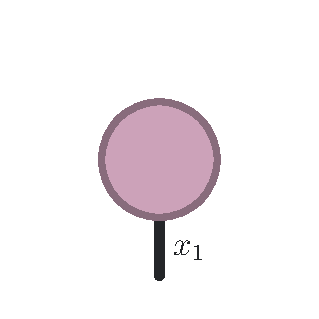
\includegraphics[width=1\textwidth]{figures/tensor-2.pdf}
        \label{fig:vqcount-circuit-b}
    \end{subfigure}
    \begin{subfigure}[h]{0.24\textwidth}
        \centering
        \caption{}
        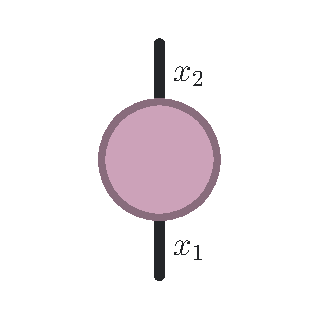
\includegraphics[width=1\textwidth]{figures/tensor-3.pdf}
        \label{fig:vqcount-circuit-b}
    \end{subfigure}
    \begin{subfigure}[h]{0.24\textwidth}
        \centering
        \caption{}
        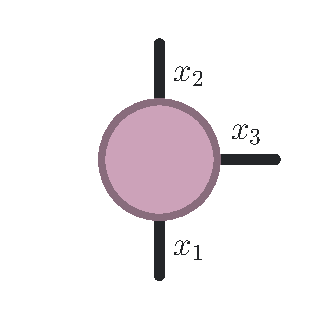
\includegraphics[width=1\textwidth]{figures/tensor-4.pdf}
        \label{fig:vqcount-circuit-b}
    \end{subfigure}
    \caption[Représentation géométrique des tenseurs]{}
    \label{fig:tensor} 
\end{figure}

Plusieurs opérations peuvent être appliquées sur les tenseurs constituants, tel qu'illustré à la figure XXX. Le \textit{produit tensoriel} entre deux tenseurs $A$ et $B$ sur les ensembles d'indices respectifs $\varepsilon_{1}$ et $\varepsilon_{2}$ correspond au produit élément par élément des valeurs des tenseurs, généralisant ainsi le produit extérieur entre deux vecteurs:

\begin{equation}
    (A \otimes B)[\varepsilon_{1}, \varepsilon_{2}] \coloneq A[\varepsilon_{1}] \cdot B[\varepsilon_{2}] \,.
\end{equation}

Le produit tensoriel se visualise simplement par la juxtaposition des deux tenseurs. La \textit{trace} (partielle) d'un tenseur $A$ est la sommation jointe sur deux indices $x_{i}$ et $x_{j}$ de $A$ ayant la même dimension $d_{x_{i}} = d_{x_{j}}$:

\begin{equation}
    \text{Tr}_{x_{i}, x_{j}} (A[x_{i}, x_{j}, \varepsilon \setminus \set{x_{i}, x_{j}}]) \coloneq \sum_{k}^{d_{x_{i}}} A[k, k, \varepsilon \setminus \set{x_{i}, x_{j}} ] \,. 
\end{equation}

Géométriquement, la trace implique de joindre les pattes du tenseur. La \textit{contraction} de deux tenseurs est l'opération la plus commune, consistant à un produit tensoriel entre deux tenseurs $A$ et $B$ suivi d'une trace entre les indices communs $\partial \varepsilon$ de ces derniers:

\begin{equation}
    C[\varepsilon \setminus \set{ \partial \varepsilon}] \coloneq  \sum_{\partial \varepsilon} (A \otimes B)[\partial \varepsilon,  \varepsilon \setminus \set{ \partial \varepsilon}]
\end{equation}

Deux tenseurs contractés se combinent alors en une seule forme géométrique avec des pattes correspondant aux indices non contractés. Comme les tenseurs ne sont en réalité que des tableaux multidimensionnels, il est possible de réorganiser l'information encodée sous une différente forme. Les opérations de \textit{regroupement} et de \textit{séparation} modifient l'organisation de cette information. Par exemple, une matrice représentée par une matrice de taille $d_{1} \times d_{2}$ peut aussi être encodée dans un vecteur de taille $d_{1} \cdot d_{2}$. Cette manipulation des données se représente graphiquement par un regroupement ou une séparation des pattes des tenseurs.

Finalement, l'opération inverse à la contraction est la \textit{décomposition}, où un tenseur est décomposé en deux différents tenseurs. Un exemple particulièrement intéressant est la \textit{décomposition en valeurs singulières}, une méthode typiquement appliquée aux matrices, mais pouvant se généraliser aux tenseurs en les regroupant sous formes de matrices. Cette décomposition permet en plus de réduire la dimension des indices et donc de retirer l'information superflue et retirant les valeurs négligeables de la matrice singulière.

Les méthodes de réseaux de tenseur suivent couramment la démarche suivante. Le problème à résoudre est modélisé sous la forme d'un réseau de tenseur en encodant les contraintes sous la forme de tenseurs, de façon à ce que la contraction de ce réseau donne la solution au problème. En utilisant les opérations précédentes, incluant potentiellement les opérations de décomposition ou de regroupement pour la simplification, le réseau est contracté pour obtenir la solution souhaitée. Notons que l'ordre de contraction, c'est-à-dire l'ordre dans lequel chacun des tenseurs est contracté avec les tenseurs environnants, à un fort impact sur la quantité de ressources nécessaires~\cite{grayHyperoptimizedTensorNetwork2021}.

%-----------------------------------------------------------------------------%

\section{État en produit de matrices et opérateur en produit de matrices}
\label{sec:mps-mpo}

Un \textit{état en produit de matrices} (« Matrix Product State ») (MPS) est type particulier de réseau de tenseurs permettant la représentation efficace d'un état quantique. Considérons un état quantique $\ket{\psi}$ à $m$ qubits. En employant la notation en réseau de tenseurs, cet état se représente par un tenseur de rang $m$, avec $m$ indices de dimensions $d=2$, encodant les amplitudes des qubits de $\ket{\psi}$. Cette représentation nécessite un grand nombre d'éléments, plus précisément $2^{n}$, pour encoder l'entièreté des amplitudes des qubits. Alternativement, ce tenseur peut être décomposé en $m$ tenseurs à l'aide de la décomposition en valeurs singulières tel qu'illustré à la figure XXX. En coupant les plus petites valeurs de la matrice singulière, correspondant à l'information redondante du système, une représentation de taille réduite peut être obtenue permettant ainsi l'étude de l'état souhaité. Les MPS sont particulièrement utile pour l'étude de l'intrication entre deux sous-parties d'un système comme celle-ci est capturée dans les indices du MPS.

Les opérateurs en produit de matrices permettent quant à eux d'appliquer un opérateur sur un MPS. La méthode MPS/MPO peut par exemple représenter l'évolution d'un système quantique selon un certain Hamiltonien (représenté sous forme de MPO).

\begin{figure}[h!]
    \centering
    \begin{subfigure}[h]{0.7\textwidth}
        \centering
        \caption{}
        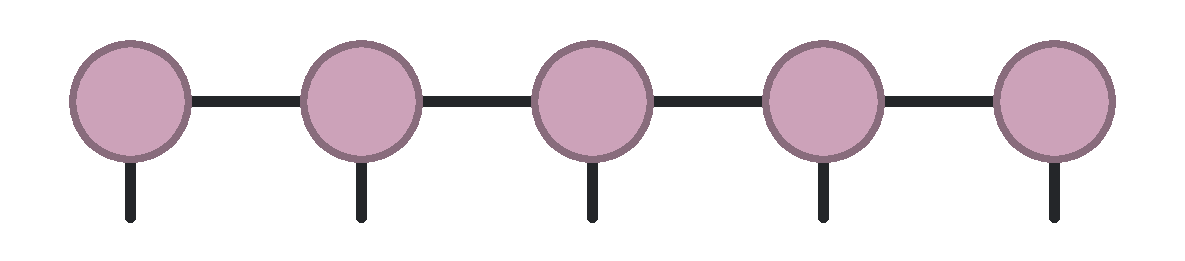
\includegraphics[width=1\textwidth]{figures/mps.pdf}
        \label{fig:vqcount-circuit-a}
    \end{subfigure}
    \begin{subfigure}[h]{0.7\textwidth}
        \centering
        \caption{}
        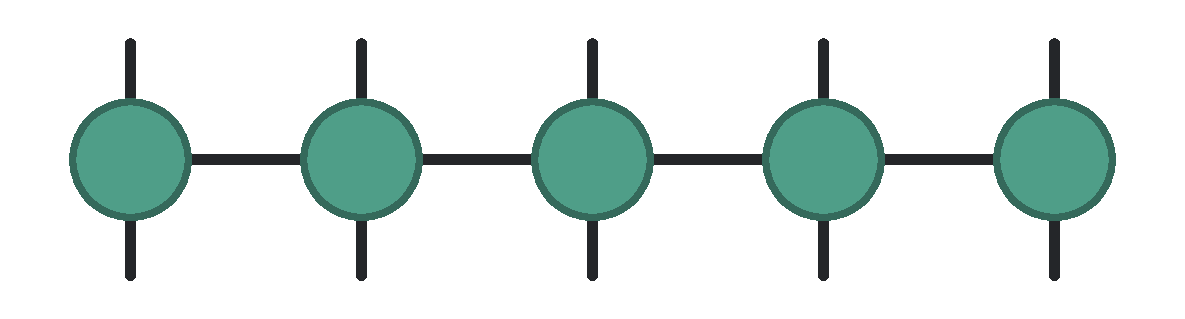
\includegraphics[width=1\textwidth]{figures/mpo.pdf}
        \label{fig:vqcount-circuit-b}
    \end{subfigure}
    \caption[État et opérateur en produit de matrices]{Schéma d'un état (a) et d'un opérateur (b) en produit de matrices.}
\end{figure}


%-----------------------------------------------------------------------------%

\section{Simulation de circuits quantiques}
\label{sec:simulation-de-circuits-quantiques}

\begin{comment}
\subsection*{Plan}

\begin{enumerate}
    \item Décrire le lien entre les circuits quantiques et les réseaux de tenseurs
    \item Décrire les différentes méthodes de simulation (MPS-MPO et réseau de tenseurs général)
    \item Décrire la méthode d'échantillonage
\end{enumerate}

\subsection*{Références}

1. Gray, J. quimb: A python package for quantum information and many-body calculations. Journal of Open Source Software 3, 819 (2018).

2. Ferris, A. J. and Vidal, G. Perfect Sampling with Unitary Tensor Networks. Phys. Rev. B 85, 165146 (2012).
\end{comment}

Les réseaux de tenseurs font partie des méthodes les plus performantes pour la simulation de circuits quantiques. En effet, un s'encode facilement par un tenseur de dimension $d = 2 \times 2$. De même, 

La méthode MPS/MPO se prête particulièrement bien à la simulation de circuit quantique. 

Afin d'obtenir des échantillons à partir d'un réseau de tenseur, deux méthodes sont possibles. D'abord, une représentation dense de la fonction d'onde peut être obtenue en contractant le réseau. Les états sont alors simplement obtenus en pigeant selon la distribution de probabilité trouvée. Une méthode alternative utilise plutôt ~\cite{ferrisPerfectSamplingUnitary2012}. 






%-----------------------------------------------------------------------------%
